% Let's start by addressing the following problem: consider a dictionary $\mathcal{D}$ of $n$ strings drawn from an alphabet $\Sigma$. We can represent the whole dictionary as a single string $T[1,m]$\footnote{Without any separator between strings} by concatenating all the strings in $\mathcal{D}$, where $m$ is the total length of the dictionary. The problem is to support the following queries:
% \begin{itemize}
%     \item \texttt{Access\_string(i)}: return the $i$-th string in $\mathcal{D}$.
%     \item \texttt{Which\_string(x)}: retrieve the starting position of the string in $T$ including
%     the symbol $T[x]$.
% \end{itemize}
% The classic approach to solve this problem is via an array of pointers A[1, n] to $\mathcal{D}$'s strings, implemented by means of their offsets in $T[1, m]$, thus using $\theta(n \log n)$ bits overall. So the operation \texttt{Access\_string(i)} boils down to returning $A[i]$, whereas \texttt{Which\_string(x)} boils down to finding the predecessor of $x$ in $A$. The first operation takes constant time, while the second one takes $O(\log n)$ time via binary search.

\todo[fancyline]{Change this introduction, I don't like it}In the previous chapter, we introduced various methods for compressing data. Now we introduce the concept of compressed data structures: data structures that store data in a compressed form, allowing for efficient access to the data. This will lead to the introduction of the so called \emph{pointer-less programming}, where we ditch the traditional pointers and instead use compressed data structures built upon binary arrays that allow for efficient access to the data. In this chapter, we will introduce the concept of bitvectors, and show how they can be compressed to support rank and select queries in constant time. We will then introduce wavelet trees, a data structure that generalizes the concept of bitvectors to support rank and select queries on arbitrary alphabets.


\section{Bitvectors}\todo[]{Maybe call this section "RRR: A succint data structure for rank and select" or something like that}
Consider the following problem \cite{ferragina2023pearls}: imagine a dictionary $\mathcal{D}$ containing $n$ strings from an alphabet $\Sigma$. We can merge all strings in $\mathcal{D}$ into a single string $T[1,m]$, without any separators between them, where $m$ is the total length of the dictionary. The task is to handle the following queries:
\begin{itemize}
    \item \texttt{Read(i)}: retrieve the $i$-th string in $\mathcal{D}$.
    \item \texttt{Which\_string(x)}: find the starting position of the string in $T$, including the character $T[x]$.
\end{itemize}
The conventional solution involves employing an array of pointers $A[1, n]$ to the strings in $\mathcal{D}$, represented by their offsets in $T[1, m]$, requiring $\Theta(n \log n)$ bits. Consequently, \texttt{Read(i)} simply returns $A[i]$, while \texttt{Which\_string(x)} involves locating the predecessor of $x$ in $A$. The first operation is instantaneous, whereas the second one necessitates $O(\log n)$ time using binary search. \vspace{0.4cm}

\noindent We can address the problem by employing a compressed representation of the offsets in $A$ via a binary array $B[1,m]$ of $m$ bits, where $B[i] = 1$ if and only if $i$ is the starting position of a string in $T$. In this case then $\texttt{Access\_string(i)}$ searches for the $i$-th $1$ in $B$, while $\texttt{Which\_string(x)}$ counts the number of $1$s in the prefix $B[1,x]$. \vspace{0.4cm}

\noindent In modern literature this two operations are well known as \textit{rank} and \textit{select} queries, respectively.
\begin{definition}[Rank and Select]\label{def:rankselect}
    Given $B[1,n]$ a binary array of $n$ bits (a bitvector), we define the following operations:
    \begin{itemize}
        \item The \textbf{rank} of an index $i$ in $B$ relative to a bit $b$ is the number of occurrences of $b$ in the prefix $B[1,i]$. We denote it as $rank_1(i) = \sum_{j=1}^{i} B[j]$. Similarly we can compute $rank_0(i) = i - rank_1(i)$ in constant time.
        \item The \textbf{select} of the $i$-th occurrence of a bit $b$ in $B$ is the index of the $i$-th occurrence of $b$ in $B$. We denote it as $select_b(i)$. Opposite to rank, we can't derive select of $0$ from select of $1$ in constant time.
    \end{itemize}
\end{definition}

\begin{example}[Rank and Select on a plain bitvector]

\end{example}
\missingfigure[]{Example of a bitvector $B[1, 20]$ with the rank and select operations.} \vspace{0.4cm}

\noindent As stated before, bitvectors are the fundamental piece in the implementation of compressed data structures. Therefore, an efficient implementation is crucial. In the following sections, our aim is to built structures of size $o(n)$ bits that can be added on top either the bit array or the compressed representation of $B$ to facilitate rank and select operations. We will see that will often encounter skewed distributions of $0$s and $1$s in $B$, and we will exploit this property to achieve higher order compression.

\begin{remark}
    If we try to compress bitvectors with the techniques seen in \autoref{ch:Chapter2}, we would need to encode each bit individually, requiring at least $n$ bits.
\end{remark}

\subsection{Rank} \label{subsec:rank}

In their seminal paper \cite{RRR2002} Raman et al. introduced a hierarchical succinct data structure that supports the rank operation in constant time, while only using \todo{or  just $o(n)$?} $n + o(n)$  bits of space. The structure is based on the idea of splitting the binary array $B[1, n]$ into big and small blocks of fixed length, and then encoding the number of bits set to $1$ in each block. \vspace{0.4cm}

\noindent More precisely, the structure is composed of three levels: in the first one we (logically) split $B[1, n]$ into blocks of size $Z$ each, where at the beginning of each superblock we store the number (\emph{class number}) of bits set to $1$ in the corresponding block, i.e the output of the query $rank_1(i)$ for $i$ being the starting position of the block. In the second level, we split the superblocks into blocks of size $z$ bits each\footnote{For simplicity, we assume that $z$ divides $Z$} with the same meta-information stored at the beginning of each block. Finally the third level is a lookup table that is indexed by the small blocks and queried positions. In other words, for each possible small block and each possible position within that block, the lookup table stores the result of the $rank_1$ operation. This pre-computed information allows for constant time retrieval of the $rank_1$ operation results, as the result can be directly looked up in the table instead of having to be computed each time. This is the key to the efficiency of the data structure. In this way, the $i-th$ block, of size $Z$, can be accessed as
\[
    B[i \cdot Z + 1, (i+1) \cdot Z]
\]
while the small block $j$ of size $z$ in the $i-th$ superblock is
\[
    B[i \cdot Z + j \cdot z + 1, i \cdot Z + (j+1) \cdot z] \qquad \forall j \in [0, Z/z), \forall i \in [0, n/Z)
\]
We will denote with $r_i$ and call it \emph{absolute rank} the number of bits set to $1$ in the $i-th$ block, and with $r_{i,j}$ (\emph{relative rank}) the number of bits set to $1$ in the $j-th$ small block of the $i-th$ superblock. Figure \ref{fig:RRR} shows a visual representation of the RRR data structure.

\begin{figure}[h]
    \begin{flushright}
        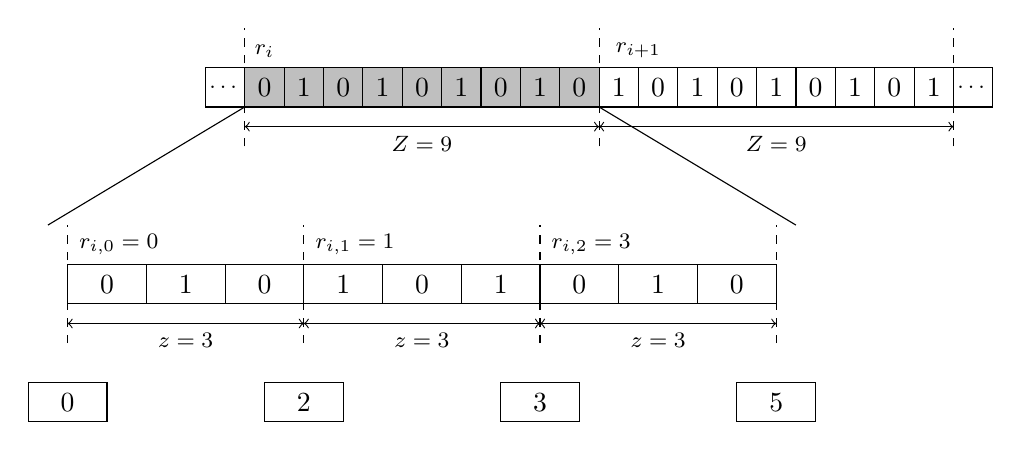
\begin{tikzpicture}[scale=0.5] % Adjust the scale as needed
            \foreach \x/\bit in {0/\footnotesize{\dots}, 1/0, 2/1, 3/0, 4/1, 5/0, 6/1, 7/0, 8/1, 9/0, 10/1, 11/0, 12/1, 13/0, 14/1, 15/0, 16/1, 17/0, 18/1, 19/\footnotesize{\dots}} {
                    \ifnum\x<1
                        \draw (\x,0) rectangle (\x+1,1) node[midway] {\bit};
                    \else
                        \ifnum\x<10
                            \draw[fill=lightgray] (\x,0) rectangle (\x+1,1) node[midway] {\bit};
                        \else
                            \draw (\x,0) rectangle (\x+1,1) node[midway] {\bit};
                        \fi
                    \fi
                }
            % Add dashed lines
            \draw[dashed] (1,-1) -- (1,2);
            \draw[dashed] (10,-1) -- (10,2);
            \draw[dashed] (19,-1) -- (19,2);

            % add double arrow
            \draw[<->] (1,-0.5) -- (10,-0.5) node[midway, below] {\footnotesize{$Z=9$}};
            \draw[<->] (10,-0.5) -- (19,-0.5) node[midway, below] {\footnotesize{$Z=9$}};

            % Add label over the blocks 2, 10
            \node[above] at (1.5,1) {\footnotesize{$r_i$}};
            \node[above] at (11,1) {\footnotesize{$r_{i+1}$}};

            % Add one line that starts from the bottom angle of block 1, and goes down inclined
            \draw[-] (1,0) -- (-4,-3);
            \draw[-] (10,0) -- (15,-3);

            \foreach \x/\bit in {0/0, 1/1, 2/0, 3/1, 4/0, 5/1, 6/0, 7/1, 8/0} {
                    \draw (\x*2-3.5,-5) rectangle (\x*2-1.5,-4) node[midway] {\bit};
                }

            % Add dashed lines
            \draw[dashed] (-3.5,-6) -- (-3.5,-3);
            \draw[dashed] (2.5,-6) -- (2.5,-3);
            \draw[dashed] (8.5,-6) -- (8.5,-3);
            \draw[dashed] (14.5,-6) -- (14.5,-3);

            % add double arrow
            \draw[<->] (-3.5,-5.5) -- (2.5,-5.5) node[midway, below] {\footnotesize{$z=3$}};
            \draw[<->] (2.5,-5.5) -- (8.5,-5.5) node[midway, below] {\footnotesize{$z=3$}};
            \draw[<->] (8.5,-5.5) -- (14.5,-5.5) node[midway, below] {\footnotesize{$z=3$}};

            % Add label over the blocks 2, 10
            \node[above] at (-2.2,-4) {\footnotesize{$r_{i,0} = 0$}};
            \node[above] at (3.8,-4) {\footnotesize{$r_{i,1} = 1$}};
            \node[above] at (9.8,-4) {\footnotesize{$r_{i,2} = 3$}};


            \foreach \x/\bit in {-4.5/0, 1.5/2, 7.5/3, 13.5/5} {
                    \draw (\x,-8) rectangle (\x+2,-7) node[midway] {\bit};
                }
        \end{tikzpicture}
    \end{flushright}
    \caption{The RRR Rank data structure, showing the three levels of the structure. The first level is composed of blocks of size $Z$, the second level of blocks of size $z$, and the third level is a lookup table.} \label{fig:RRR}
\end{figure}

\noindent Let's focus on the third level: the lookup table. Along with the value of the absolute and relative ranks, we also store an offset that serves as an index into the table. To be precise, this table is a table of tables: one for each possible value of $r_i$ and $r_{i,j}$. The table $T$ is then indexed by the values of $r_i$ and $r_{i,j}$. For every possibile value of $r_i$ and $r_{i,j}$, the sub-table stores an array of cumulative sums. Thus, since we have $\binom{Z}{z}$ possible values for $r_i$ and $r_{i,j}$ (and consequently entries in the considered sub-table), the lookup table has a size of $\binom{Z}{z}\log Z$ bits. In Table \ref{tab:lookup} we show an example of a lookup table for the RRR data structure. \vspace{0.4cm}

\begin{table}[h]
    \centering
    \begin{tabular}{|c|c|c|c|}
        \hline
        \textbf{block} & $\mathbf{r_{i,0}}$ & $\mathbf{r_{i,1}}$ & $\mathbf{r_{i,2}}$ \\
        \hline
        000            & 0                  & 0                  & 0                  \\
        001            & 0                  & 0                  & 1                  \\
        010            & 0                  & 1                  & 1                  \\
        011            & 0                  & 1                  & 2                  \\
        100            & 1                  & 1                  & 1                  \\
        101            & 1                  & 1                  & 2                  \\
        110            & 1                  & 2                  & 2                  \\
        111            & 1                  & 2                  & 3                  \\
        \hline
    \end{tabular}
    \caption{Example of a lookup table $T$ for the RRR data structure. The table stores the result of the rank operation for all possible small blocks with $z = 3$. The cell $T[b, r_{i,j}]$ stores the result of the rank operation for the block $b$ inside the $i-th$ superblock and the $j-th$ small block.} \label{tab:lookup}
\end{table}

\noindent We can now state the following theorem:

\begin{theorem} \label{th:rank}
    The space occupancy of the Rank data structure is $o(n)$ bits, and thus it is asymptotically sublinear in the size of the binary array $B[1, n]$. The Rank algorithm takes constant time in the worst case, and accesses the array $B$ only in read-mode
\end{theorem}
\begin{proof}
    The space occupancy of all the big blocks can be computed by multiplying the number of big blocks by the number of bits needed to store the \emph{absolute rank} of each block. Thus, the space occupancy of the big blocks is $O(\frac{n}{Z} \log m)$ bits, since each block can store at most $m$ bits. The same reasoning can be applied to the small blocks, which occupy $O(\frac{n}{z} \log Z)$ bits, since each block can store at most $Z$ bits. So the space complexity is
    \begin{equation}
        O\left(\frac{n}{Z} \log m + \frac{n}{z} \log Z\right)
    \end{equation}
    Let's set $Z = (\log n)^2$ and $z = 1/2 \log n$, then the space complexity becomes
    \begin{align}
         & = O\left(\frac{n}{(\log n)^2} \log m + \frac{n}{\frac{1}{2} \log n} \log (\log n)^2\right) \\
         & = O\left(\frac{n}{\log^2n} \log m + \frac{n}{\log n} \log \log n\right)                    \\
         & = O\left(\frac{n \log \log n}{\log n} \right)= o(n)
    \end{align}
\end{proof}

\noindent The current explanation of this data structure only clarifies how to respond to rank queries for indices located at the end of a block (or superblock). This can be achieved efficiently, taking constant time, either by directly accessing the value in the lookup table or by calculating the cumulative rank of preceding blocks along with the relative rank within the current block. \vspace{0.4cm}

\noindent However, we also need to address the non-trivial case where the index $i$ is located in the middle of a block\footnote{For the sake of simplicity, we will assume that $B[x]$ is included in the $j-th$ small block of the $i-th$ superblock}. Differently from the previous case, if we want to compute the $rank_1$ operation over an arbitrary position $x$, we would need to compute $r_i + r_{i,j} + \texttt{popcount}(B_{i,j}[1,x])$, where the last term is an operation that counts the number of bits set to $1$ in the prefix $B_{i,j}[1,x]$. While the first two terms can be computed in constant time, the last term requires $O(\log n)$ time\footnote{It actually grows log-logarithmically with the size of the small blocks} in the worst case.

\begin{remark}
    If $z$ (the size of the small blocks) can be stored in a single memory word, the \texttt{popcount} operation can be executed efficiently using bit manipulation operations like \texttt{std::popcount} in C++\footnote{https://en.cppreference.com/w/cpp/numeric/popcount}. This approach ensures constant time execution, especially when $z$ occupies only a few memory words, allowing for the utilization of SIMD (single instruction, multiple data) operations for faster performance. \cite{ferragina2023pearls}
\end{remark}

\noindent If the size of the small blocks doesn't fit in a single memory word, we can pre-process in our lookup table (the third level of the data structure) all the results of the \texttt{popcount} operation for all possible blocks and then use this table to answer rank queries in constant time (as shown in table \ref{tab:lookup}). Let's denote this table as $T$ and see how to use it to answer rank queries in constant time. In order to retrive the result of $\texttt{popcount}(B_{i,j}[1,x])$ we can access the table $T$ at the position $T[B_{i,j}, o]$. Where $o$ is the offset of the bit $B[x]$ in $B_{i,j}$, and $B_{i,j}$. The offset $o$ can be computed as $o = 1 + ((x-1) \mod z)$. Thus we only need to perform three atomic operations, two memory accesses and one addition, to retrieve the result of the rank operation in constant time. \vspace{0.4cm}

\noindent Storing this table requires $O(\sqrt{n} \log \log n)$ bits\footnote{We have $2^z$ rows and $z$ columns and each cell stores a value in $[0, z]$.}, which is asymptotically sub-linear in the size of the binary array $B[1, n]$ and allows the \texttt{popcount} operation in a block of $O(\log n)$ bits in constant time. Thus, if we consider the word length as $\log n$ and still maintain the $o(n)$ space occupancy stated in \ref{th:rank}  \vspace{0.4cm}

\todo[inline, color=blue!30]{TBD: Do I talk about \cite{grossi2009haste}?}

\begin{remark}[Pratical Considerations]\todo[fancyline]{Improve this, I think there are errors}
    Optimizing memory access can significantly boost performance: thus aligning block and superblock lengths to word or byte boundaries is crucial. For instance, setting the superblock length ($Z$) to $256$ allows storing the second level as an array of $\lceil n/z \rceil$ bytes, resulting in a total space usage of $1.375 \cdot n$ for both $z = 32$ and $z = 64$. To further minimize space overhead, introducing another level with super-superblocks of length $2^{16}$ can bring down the total space usage to below $1.313 \cdot n$ for $z = 32$ and $1.189 \cdot n$ for $z = 64$. To reduce cache misses, interleaving the secondo and the third level ensures that the accessed entries from both arrays fit in the same cache line, enhancing performance. For example, with $z = 64$, choosing $n/Z = 8$ allows storing two w-bit words per superblock, minimizing space usage to $1.250 \cdot n$. \cite{navarro2016compact}
\end{remark}

% \noindent Algorithm \ref{alg:rank} shows the Rank algorithm, which takes as input the binary array $B$ and an index $i$, and returns the rank of the bit at index $i$ in $B$. For the sake of simplicity, we will use some C++ methods from the standard library: in particular, we will use the method \texttt{std::popcount}\footnote{https://en.cppreference.com/w/cpp/numeric/popcount} that returns the number of bits set to $1$ in a given integer.

% \begin{algorithm}[h]
%     \begin{algorithmic}[1]
%         \Function{Rank}{$B,i$}
%         \State $Z \gets \log^2 n$
%         \State $z \gets \frac{1}{2} \log n$
%         \State $i \gets \lfloor i / Z \rfloor$
%         \State $j \gets \lfloor i / z \rfloor$
%         \State $r_i \gets \text{absolute rank of block } i$
%         \State $r_{i,j} \gets \text{relative rank of block } j \text{ in superblock } i$
%         \State $o \gets 1 + ((i \cdot Z + j \cdot z) \mod z)$
%         \State \Return $r_i + r_{i,j} + T[B[i,j], o]$
%         \EndFunction
%     \end{algorithmic}
%     \caption{Rank Algorithm} \label{alg:rank}
% \end{algorithm}


\subsection{Select}
The $select$ operation can be seen as the inverse of the rank operation, i.e given a binary array $B$ and an integer $i$, the $select$ operation returns the index of the $i$-th occurrence of a bit $b$ in $B$. More formally, we have that:
\[
    rank_c(B, select_c(B, i)) = i
\]
The implementation of the select operation heavily relies on the three level data structure discussed before (\ref{subsec:rank}). The difference lies in the fact that, in this case, the bitmap $B$ doesn't get split into blocks of fixed size, but rather into blocks of variable size that are determined by the rank of the block.
























\subsection*{Do I talk about the elias fano version?}
\todo[inline, color=blue!30]{Do I talk also about how to compress via Elias Fano? When the numbers of $1s$ in B is much smaller than $n$, where I can achieve $n\mathcal{H}_0(B) + O(m)$ bits of space occupancy. This approach poses a much lower overhead over the entropy. It supports $Select$ in constant time, while $access$ and $Rank$ in $O(\log \frac{n}{m})$ \cite{navarro2016compact,ferragina2023pearls}. On a further note, in \cite{FERRAGINA2007115} Ferragina and Venturini achieved higher order compression for general strings, supporting access in constant time (so adding rank and select for bitvectors are natural extensions), do I talk about this as well?}
